\documentclass[10pt,a4paper]{article}
\usepackage[margin=2.2cm]{geometry}
\usepackage[T1]{fontenc}
\usepackage[utf8]{inputenc}
\usepackage{lmodern}
\usepackage{microtype}
\usepackage{amsmath,amssymb}
\usepackage{graphicx}
\usepackage{booktabs}
\usepackage{xcolor}
\usepackage{caption}
\usepackage{enumitem}

\usepackage[numbers,sort&compress]{natbib}
\usepackage[hidelinks]{hyperref}
\graphicspath{{figures/}}
\setlist{nosep,leftmargin=1.4em}
\captionsetup{font=small,labelfont=bf}
\setcitestyle{authoryear,open={(},close={)}}
\newcommand{\bpb}{bits/byte}
\newcommand{\figw}{\linewidth}

\title{Training small language models under computational constraints\\[2pt]
\large Investigating how domain share affects model effectiveness in a narrow-domain}
\author{Jacob Seng Keng Hui, A0273790W}

\begin{document}
\maketitle

\section*{Code Availability}
The code, data preparation scripts, and run configurations required to reproduce all experiments in this paper are available at \url{https://github.com/R0bocat/DSA4212}.\\

\noindent\fbox{\parbox{\dimexpr\linewidth-2\fboxsep-2\fboxrule\relax}{%
\textbf{Declarations:}
\begin{description}[leftmargin=0.6em,labelindent=0pt,style=nextline]
\item[Compute budget.] All runs (unless specified) were trained with a budget of 300M training tokens (approximately 41 minutes of 
compute time using RX 6900XT (16GB) GPU) Each training run was hard capped at 45 minutes but none of them were truncated by
this time limit. A token budget was picked over elapsed real time as it makes the result more compareable and isolated from
any potential hardware issues.
\item[Initialisation.] Every model initializes with normally-distributed weights $(\mathcal{N}\sim(0,0.02^2))$ with residual projections scaled 
by $\frac{0.02}{\sqrt{2L}}$ as per the nanogpt architecture. Most of the language model architecture was taken from nanogpt and 
modified to integrate data mixing. A single byte-level BPE tokenizer was trained from scratch using the train-split data, using an equal byte mix of the domain and general data to ensure that tokenizer efficiency does not impact the results of data-mixing.
\item[Evaluation objective.] The models were evaluated on held-out bits per byte (bpb) on primarily PubMed abstracts (target domain) and
secondarily on FineWeb-Edu documents (general domain), calculated as bpb $=\frac{\bar{\ell}}{\ln 2} \times \text{tokens per byte}$,
where $\bar{\ell}$ is the mean loss of nats per token. Bits per byte was chosen as it is comparable across tokenizers and is on the same scale across corpora, which is more favourable since the ratio of domain to general data changes across runs. During the training process, weights are selected based on validation data and are finally evaluated on a separate test data set.
\end{description}}}

\section{Introduction}
\paragraph{}When deciding what to do for this assignment, I thought of how language models are slowly becoming more prevalent for specific use cases, such as the use of AI in law or in medicine etc. The naive thought to training a model in the narrow domain would be to use only data from that domain. Doing a bit of research, I discovered that currently, one of the main strategies is to pretrain a general model and then finetune the model for the specific use case. I came across a paper where \citep{spt2026} mixes the small domain dataset into the general pretraining to reduce the amount of pretraining needed. I wondered if the inverse would also be true, that if I am training a model for a narrow use case, would introducing general data into the training dataset lead to better model performance or would it be better to stick to domain specific data, and if so, would there be an optimal ratio of domain-specific to general training data.


\paragraph{Research question.} At a fixed computation budget, how much does general text help small model performance in the narrow domain? 
\subparagraph{Further questions:}
\begin{itemize}
    \item Does the answer depend on how much unique data exists for the domain (U)?
    \item Is there a difference when adjusting the ratio of domain to general training data ($\delta$)? 
    \item Does the similarity of the general data to the domain data play a role?
\end{itemize}



\paragraph{Hypotheses.}
\begin{itemize}
\item \textbf{H1.} Introducing general data improves model performance in the narrow domain.
\item \textbf{H2.} The benefit of mixing in general data decreases as the domain data becomes more abundant.
\item \textbf{H3.} There is an optimal $\delta^*$ where introducing more general data would hurt the model.
\item \textbf{H4.} General data that is more similar to the domain data would improve performance more.
\end{itemize}


\section{Experimental setup}
\subsection{Data}
\paragraph{Domain: PubMed abstracts.} Used six training shards from PubMed Abstracts/train/; taken from ArmelR/the-pile-splitted mirror on Hugging Face; Licence: Mixed/per-component \citep{gao2020pile}
The data was then lightly filtered, removing duplicates, paragraphs that are likely not in english (by detecting presence of stopwords) and paragraphs that were too short. The documents were then split into train, validation and test by a
deterministic hash; validation and test contain about 1.1M tokens each while train contains about 550M tokens.

\paragraph{General: FineWeb-Edu.} For the FineWeb data, it was taken from HuggingFaceFW/fineweb-edu and the shard used was sample/10BT/000$\_$00000.parquet; License: ODC-By 1.0 \citep{penedo2024fineweb} which contains about 430M tokens. It went through the same light filtering and also was deduplicated with the PubMed data in case there was any overlapping files. Only two fully duplicated abstracts was found and removed before any run.

\paragraph{Scarcity.} The domain corpus available to a run is the first $U$ tokens of the (shuffled) PubMed training
stream, $U\in\{1,3,10,20,40\text{M}, \text{all}\approx 550\text{M}\}$, and the number of passes the model makes over the domain corpus is defined as $E=\delta \frac{B}{U}$, where B is the token budget.

\subsection{Tokenizer}
One byte-level BPE tokenizer \citep{sennrich2016bpe,radford2019gpt2} with 8192 tokens was trained on an equal-bytes sample
(400\,MB each) of PubMed and FineWeb-Edu training text and used for every reported run, so the tokenizer cannot favour
either corpus. It encodes 4.15 bytes/token on PubMed and 3.86 on FineWeb-Edu. A smaller tokenizer was chosen, 8192, rather than the typical 50k-vocabulary tokenizer because as \citep{tao2024scaling} showed, the vocabulary size should scale to the model size, and since each model's preset are small, we scaled the vocabulary down to match.


\subsection{Model, optimisation and training}
\begin{table}[h]\centering\small
\begin{tabular}{@{}ll@{}}\toprule
Architecture & 6 layers, 6 heads, width 384, MLP $4\times$ (GELU), pre-LayerNorm, tied embeddings, context 256 \\
Parameters & 13.87M (vocabulary 8192) \\
Optimiser & AdamW \citep{loshchilov2019adamw}, $\beta=(0.9,0.95)$, weight decay 0.1 on matrices, gradient clipping 1.0 \\
Learning rate & peak $10^{-3}$, 2\% warmup, cosine decay to 10\% of peak \\
Batch & 32 sequences $\times$ 256 tokens = 8192 tokens/step; 36,621 steps for 300M tokens \\
Precision & fp16 autocast with loss scaling (bf16 was 7--11$\times$ slower on this GPU) \\
Regularisation & none for the main grid; dropout 0.1-0.3 was added later on for regularisation effects\\
Evaluation & every 2000 steps on validation data; test numbers are taken at the best-validation checkpoint \\
\bottomrule\end{tabular}
\caption{Fixed settings of all main runs (nanoGPT-style decoder \citep{karpathy2022nanogpt}).}
\end{table}

\subsection{Experimental design and statistics}
\paragraph{Mixture grid.} The main experiment consists of a grid of $U\in\{3,10,40\text{M},\text{all}\}$ with $\delta\in\{0.03,0.1,0.3,0.6,1\}$ at 300M tokens, where the training sequence is drawn from the domain corpus (PubMed abstracts) with probability $\delta$ and from FineWeb-Edu otherwise. This primary grid was supported by additional runs of four kinds. Firstly, there were domain-only baseline runs that gave the grid a fair benchmark to compare against. Secondly, dropout regularisation was included for baseline and mixture runs to ensure proper tuning. Thirdly, more specific targeted runs at $U=1M$ and $20M$, finer $\delta$ values and a $150M$ token horizon were added to gain more insight. Lastly, a set of runs were performed to test if the similarity of the general data to the domain data had any impact. In total, 108 runs were completed.

\paragraph{Baselines.} Domain-only runs may stop early and each gets its own full learning-rate schedule, at $1\times$ and $2\times$ the base rate, with and without dropout. This differs from the $1.0\delta$ runs which simply continue overtraining the data until the 300M token budget. The general-only runs are also a baseline for every $U$.

\paragraph{Noise.} Pooled seed standard deviation $0.0034$~\bpb{} (14 degrees of freedom, 7 cells with repeats). A difference between two single runs therefore needs about $0.0095$~\bpb{} ($2\sigma\sqrt{2}$) to be statistically significant. Since most of the cells are single-seed, choosing the best configuration may be optimistic and could be
$0.003$--$0.005$~\bpb{} better than what it would achieve on average.

\section{Results}
\subsection{When does general data help? Scarcity and the crossover}\label{sec:grid}
\paragraph{}We first compare the standard mixture configurations (without dropout) against domain-only baselines, allowing the latter to use dropout where it improves performance. This provides a relatively strong benchmark for evaluating whether introducing general data offers an advantage over domain-specific training alone. However, this comparison does not isolate the effect of data mixing from regularisation, since the two approaches use different training configurations. We therefore conduct additional dropout experiments in Section 3.2, allowing both approaches to use regularisation for a more controlled comparison.

\begin{figure}[h]\centering
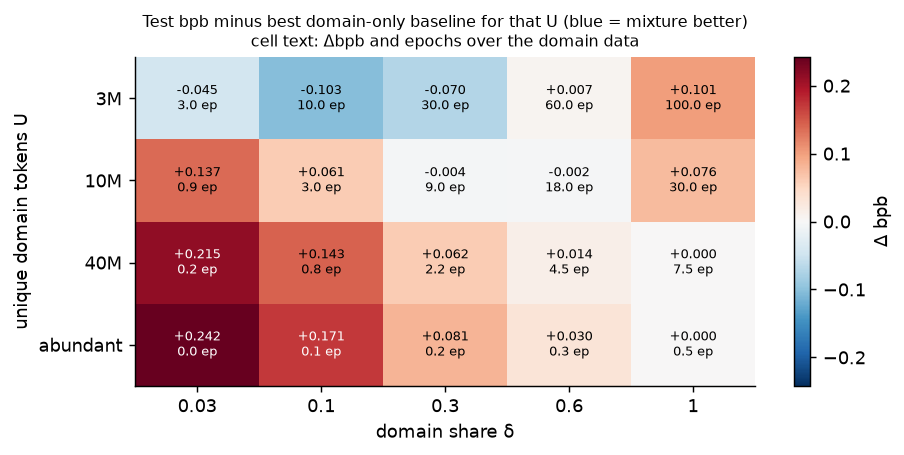
\includegraphics[width=\figw]{fig4_heatmap.png}
\caption{Gain over the best domain-only baseline for every $(U,\delta)$ cell with no dropout. Mixture runs use no dropout while domain-only baselines may use dropout. Small annotations indicate the number of domain-data passes. Bold boxes indicate the best mixture configuration.}
\label{fig:heat}
\end{figure}
\begin{table}[h]\centering\small
\begin{tabular}{@{}lllllr@{}}\toprule
$U$ & best baseline & \bpb{} & best mixture & \bpb{} & gain \\\midrule
3M & domain-only, 30 ep, dropout 0.1 & 1.309 & \(\delta=0.3\) & 1.206 & \(+0.103\) \\
10M & domain-only, 30 ep, dropout 0.1* & 1.097 & \(\delta=0.3\) & 1.091 & \(+0.004\) \\
40M & domain-only, 7.5 ep* & 1.016 & \(\delta=0.6\)* & 1.031 & \(-0.014\) \\
all (550M) & domain-only, 0.5 ep & 0.990 & \(\delta=0.6\) & 1.020 & \(-0.030\) \\ 
\bottomrule
\end{tabular}
\caption{Best baseline vs best standard (no-dropout) mixture (test \bpb{}). Baselines are the domain-only runs for each \(U\) where dropout is allowed for better regularizations. Entries marked with * are the average of 3 seeds.}
\label{tab:gain_nodropout}
\end{table}

\newpage
Figure~\ref{fig:heat} and Table~\ref{tab:gain_nodropout} show the result for the main experiment. For $U$ of 10M and 40M, runs were repeated and averaged for the result to be more statistically significant as the gain was close to the noise level. The gains are prominent for 3-10M but after a certain level of $U$, mixing in general data only hurts the performance of the model. This answers and agrees with \textbf{H2} since gain decreases and becomes negative at some point. At the same time is also disagrees with \textbf{H1} as mixing in general data seems to hurt model performance when there isn't enough passes over the domain data. 


\subsection{Fair baselines and dropout}\label{sec:baselines}
\begin{figure}[h]\centering
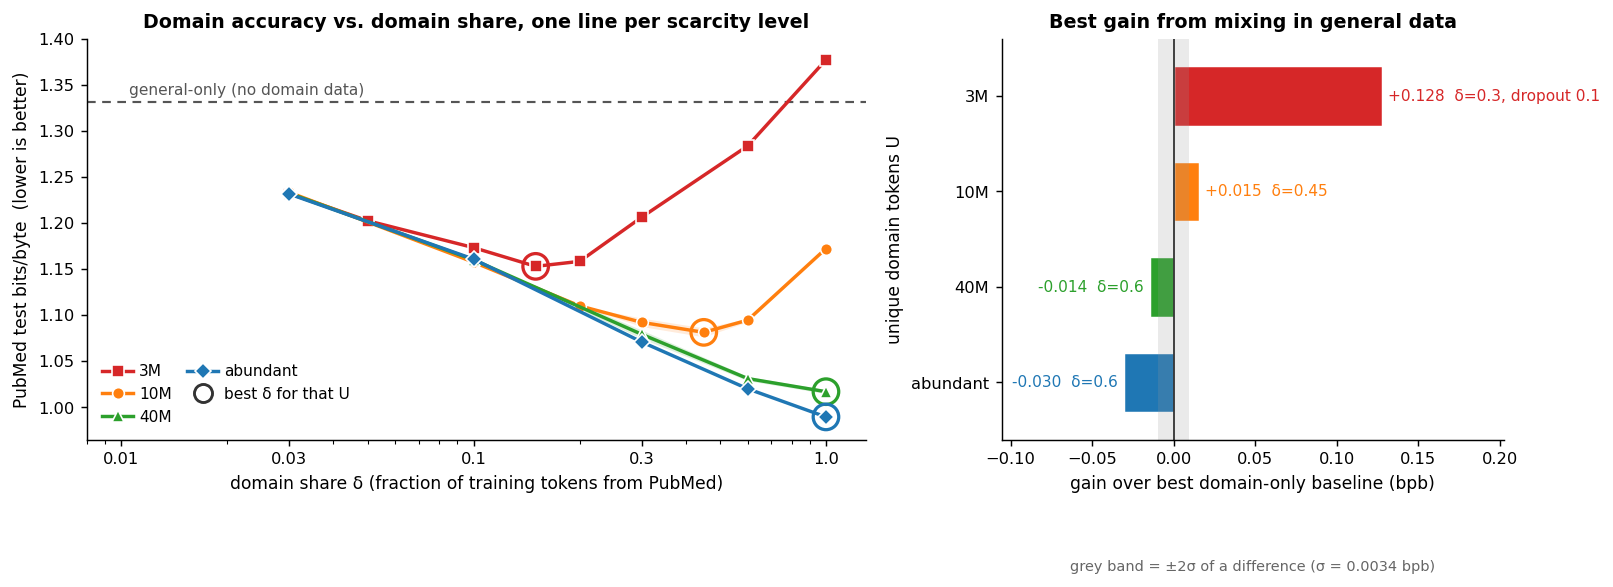
\includegraphics[width=0.85\linewidth]{fig1_main.png}
\caption{\textbf{Left:} PubMed test \bpb{} against domain share $\delta$ for each amount of unique domain data $U$. The circles mark the which is the best $\delta$, and the dashed line is the general-only run.
\textbf{Right:} Visualization of the gain of the best mixture over the best non-mixture baseline for each $U$ (grey band: $\pm2\sigma$ of a difference).}
\label{fig:main}
\end{figure}

\begin{table}[h]\centering\small
\begin{tabular}{@{}lllllr@{}}\toprule
$U$ & best baseline & \bpb{} & best mixture & \bpb{} & gain \\\midrule
3M & domain-only, 20 ep, dropout 0.1 & 1.277 & $\delta=0.3$, dropout 0.1 & 1.149 & $+0.128$ \\
10M & domain-only, 30 ep, dropout 0.1* & 1.097 & $\delta=0.45$* & 1.081 & $+0.015$ \\
40M & domain-only, 7.5 ep* & 1.017 & $\delta=0.6$* & 1.031 & $-0.014$ \\
all (550M) & domain-only & 0.990 & $\delta=0.6$ & 1.020 & $-0.031$ \\\bottomrule
\end{tabular}
\caption{Best non-mixture baseline vs best mixture (test \bpb{}; both sides may use dropout). All entries marked with * are the average of 3 seeds.}
\label{tab:gain}
\end{table}

\paragraph{}In Figure~\ref{fig:main}, the left shows how an increase in $\delta$ increases model performance, but there reaches a point of saturation when there is a lack of unique domain data and repeated training leads to worse performance. Additional runs were also performed when there was a plateau which motivated further searching for the optimal $\delta$. 
Table~\ref{tab:gain} in comparison to Table~\ref{tab:gain_nodropout} shows that adding dropout improves performance when there is heavy repetition of the domain data. This is most apparent from U=3M where the best mixture went from $\delta=0.1$ to $\delta = 0.3$ which suggests that adding dropout helps to compensate for this repetition. From the full set of runs, when mixtures have $E\geq18$, adding dropout to the model improves the \bpb{} over the dropout disabled runs but when $E\leq10$, adding dropout hurts model performance. 
\paragraph{} From the right of Figure~\ref{fig:main}, the improvements for U=3M are substantially larger than the noise, suggesting that there is strong evidence for the benefit of mixing data. However, the improvement is smaller for U=10M and the deterioration for U=40M and U=abundant are also larger than the noise threshold, suggesting that mixing in general data is detrimental when there is an abundance of unique domain data.


\newpage
\subsection{Repetition and where the optimum sits}\label{sec:rep}
\begin{figure}[h]\centering
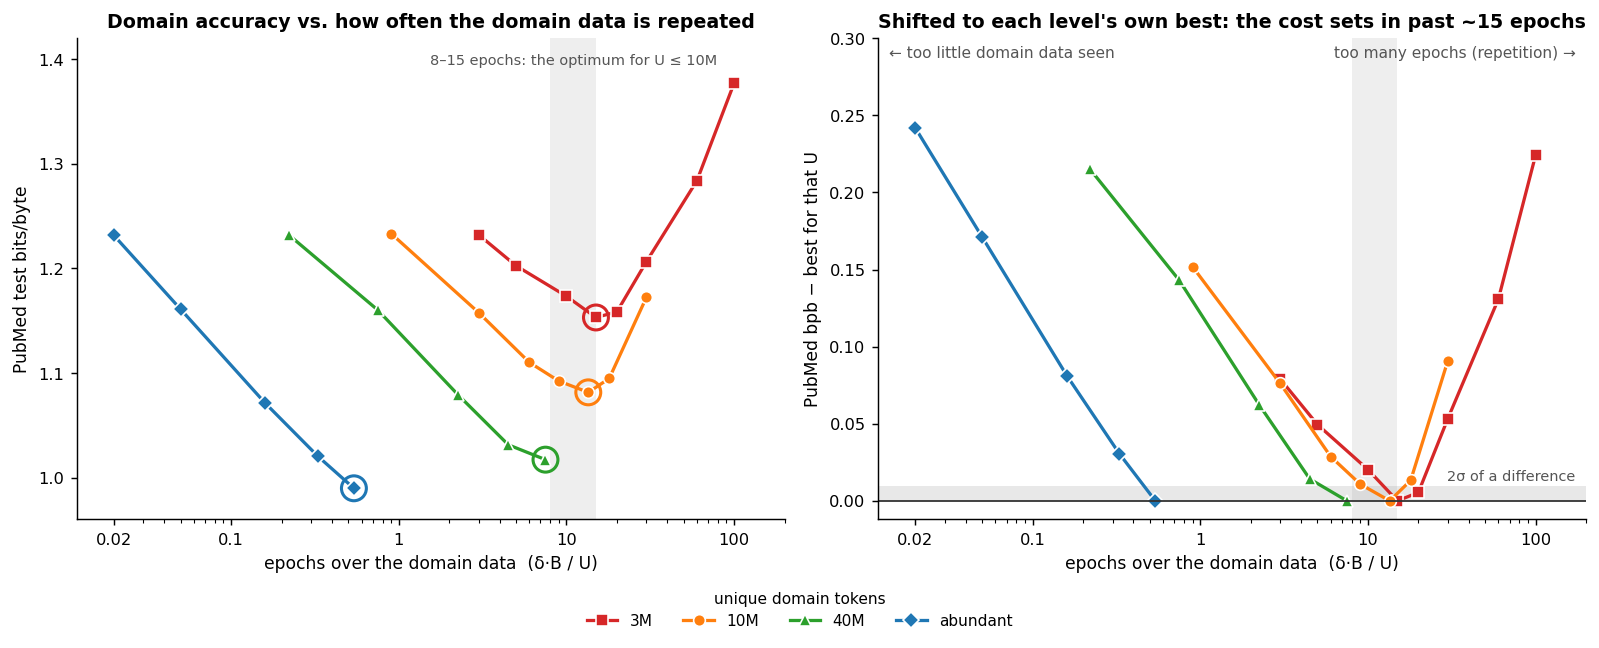
\includegraphics[width=0.85\textwidth]{fig3_repetition.png}
\caption{\textbf{Left:} PubMed test \bpb{} against passes over the domain data ($E$). \textbf{Right:} the same curves vertically shifted to where each curves best is at 0. The penalty sets in around 10--18 epochs for $U\le10$M; for $U\ge40$M the largest tested $\delta$ is still the best, so no penalty side is observed.}
\label{fig:rep}
\end{figure}
\begin{figure}[h]\centering
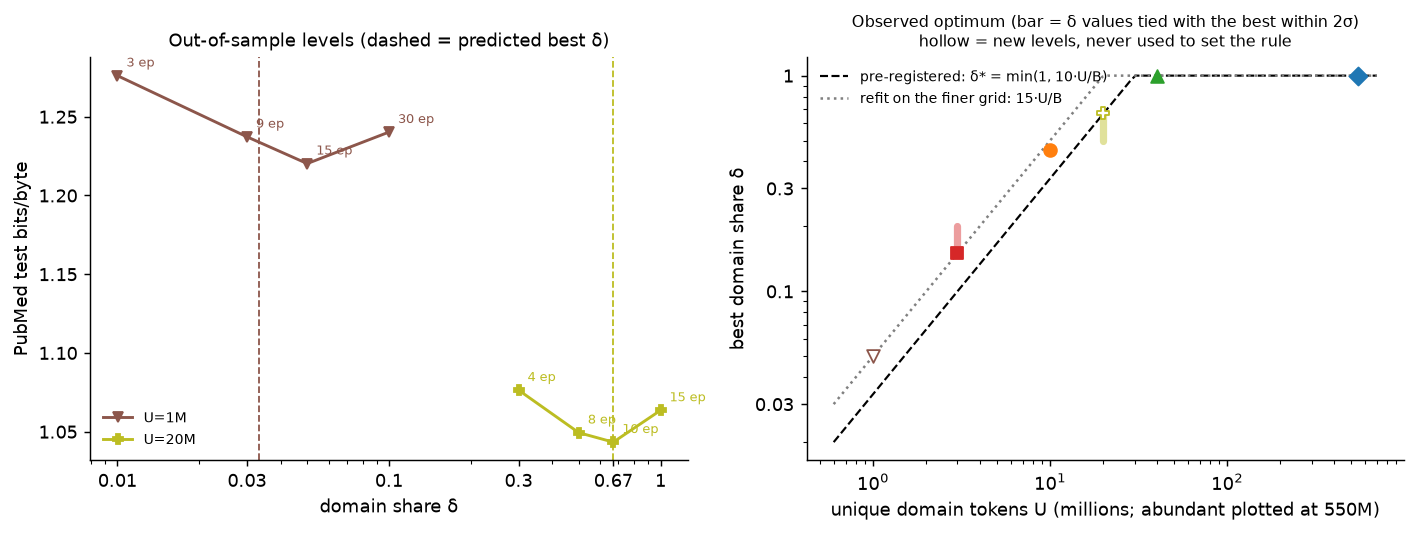
\includegraphics[width=0.85\textwidth]{fig5_rule.png}
\caption{Left: The two scarcity levels not used to set the rule, with its predicted $\delta^*$ (dashed) used to test whether the optimal level of epochs hold. Right: observed optimum for in-sample levels (bar: all $\delta$ within $2\sigma$ of the best) against the average E with error bars.}
\label{fig:rule}
\end{figure}

\paragraph{} For Figures~\ref{fig:rep} and ~\ref{fig:rule} the results are for runs without dropout since as shown above, dropout helps to mitigate the effects of repetition. 
\paragraph{}Figure~\ref{fig:rep} shows how the various $\delta^*$ seem to converge to a certain band, that when adjusting them to the graph on the right, the optimal points are at similar $E$. Figure~\ref{fig:rep} also shows the relationship between $E$ and \bpb{} where running more epochs over the domain data improves the model up till a certain threshold (around 15 epochs) before sharply resulting in additional loss for the model. 
\paragraph{} For Figure~\ref{fig:rule}, we tested two levels of scarcirty U=1M and 20M which were not sampled previously to see if the optimal delta was also found at $E^*\in[13-17]$. For the case of U=1M, the prediction was accurate however for U=20M the relationship did not hold. This could suggest that $E^*$ is not a constant value and that at some level of U, the large number of epochs over the domain data is no longer necessary. 

\begin{figure}[h]\centering
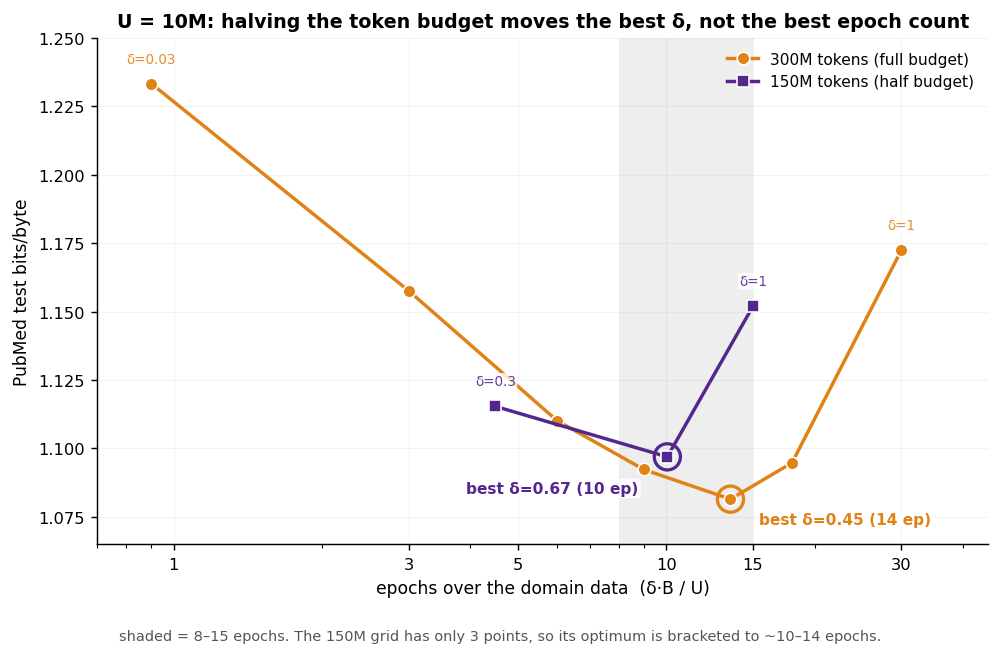
\includegraphics[width=0.7\linewidth]{fig6_horizon.png}
\caption{$U=10$M at 300M and 150M training tokens. The 150M grid has only three points (best $\delta=0.67$), so the best epoch count may not be exact.}
\label{fig:horizon}
\end{figure}

\newpage
\paragraph{}Figure~\ref{fig:horizon} introduces a model at half the computation budget. The optimal $\delta^*$ also sits nearby to the observed $E^*$ which highlights that the optimal mixture is not based on U but rather on $E$, that the model's optimal level occurs at some saturation level of epochs over the domain data. This answers \textbf{H3}, where instead of there being a $\delta^*$ for all levels of data scarcity, there is an optimal $E^*$ which accounts for compute budget and scarcity of domain data.


\subsection{Does the similarity of the general data matter?}\label{sec:sim}
\paragraph{}To test for similarity, we used a method from \cite{moore2010selection}, where each FineWeb-Edu document was scored on their first 256 tokens using two baseline models (two abundant U models with $\delta$ 0 and 1 respectively). Then using the following formula, $\text{NLL}_{\text{general-only}}-\text{NLL}_{\text{PubMed-only}}$ the documents were sorted and cut into equal-token pools. Then every pool was run at two levels, $U=10$M, $\delta=0.3$ and $U=3$M, $\delta=0.1$ with everything else unchanged. A random pool was also added as a control.

\begin{table}[h]\centering\small
\begin{tabular}{@{}lrrrrrr@{}}\toprule
 & \multicolumn{2}{c}{U=10M, \(\delta=0.3\)} & \multicolumn{2}{c}{U=3M, \(\delta=0.1\)} & & \\
pool & domain & general & domain & general & similarity & tokens \\\midrule
q1 (top quartile) & 1.0669 & 1.3844 & 1.1127 & 1.3570 & \(-0.46\) & 215M \\
q2 & 1.0936 & 1.3433 & 1.1870 & 1.3301 & \(-0.99\) & 215M \\
random & 1.0924 & 1.3416 & 1.1690 & 1.3212 & \(-1.12\) & 215M \\
q3 & 1.1061 & 1.3447 & 1.2075 & 1.3279 & \(-1.29\) & 215M \\
q4 (bottom quartile) & 1.1146 & 1.3553 & 1.2275 & 1.3471 & \(-1.74\) & 215M \\\bottomrule
\end{tabular}
\caption{Test \bpb{} by general pool. For U=10M, $\delta=0.3$: mean of 2 seeds. For U=3M, $\delta=0.1$: 1 seed. 
Similarity is the mean score of the pool according to formula. (PubMed's own documents score $+0.95$ and an average FineWeb-Edu document $-1.10$. This distribution of pools can be seen in Figure~\ref{fig:dist} in the appendix.)}
\label{tab:pools}
\end{table}

\begin{figure}[h]\centering
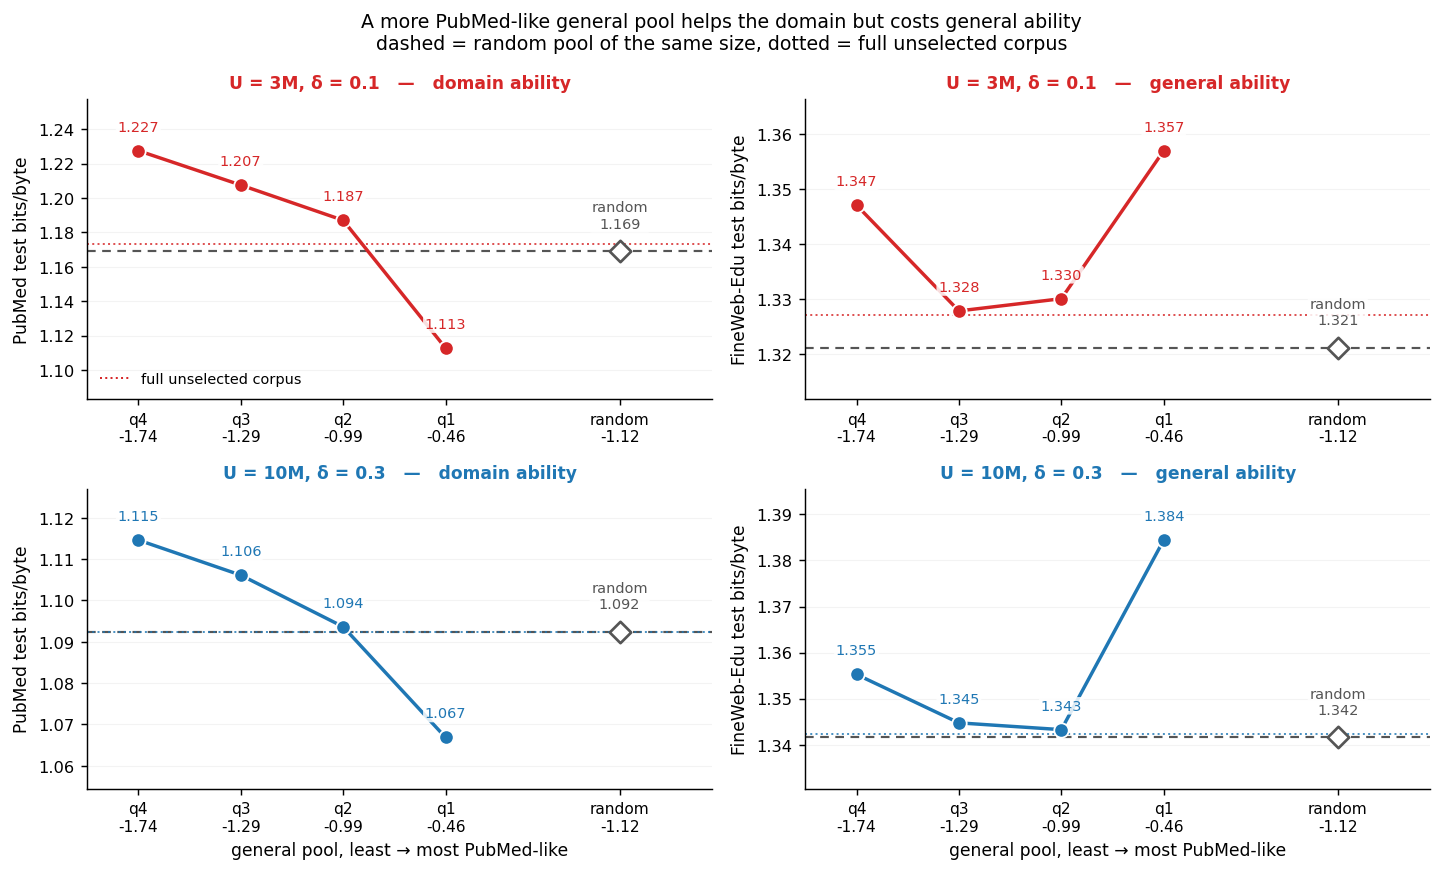
\includegraphics[width=\figw]{fig7_similarity.png}
\caption{Domain and general test \bpb{} for general pools ordered from least to most PubMed-like (pool similarity under each label). Dashed: random pool of the same size. Dotted: the full unselected corpus.}
\label{fig:sim}
\end{figure}

\newpage
\paragraph{}Figure~\ref{fig:sim} and Table~\ref{tab:pools} suggest that there is a negative correlation between domain \bpb{} and similarity. Across 8 pools, there seems to be an approximately linear relationship ($R^2\approx0.97$) with slope -0.038 per nat. This supports \textbf{H4} which suggests that more similar general data would be more useful for improving model performance. Moreover, it lines up with previous analysis where if there is an abundance of unique domain tokens, it would be better to use domain-specific data over general data.

\paragraph{} However, this relationship should be taken cautiously since it was only done at two scarcity levels and with 4 pools. Furthermore, there is an outlier at U=3M, where q2 performs worse than the random pool which has a lower similarity, which suggests that similarity alone cannot fully explain the observed differences. 

\paragraph{}For general-domain performance, the random pool consistently outperforms the similarity-selected pools. One possible explanation is that selecting increasingly domain-specific documents reduces the diversity of the training distribution, negatively affecting general language modelling. However, since diversity was not directly measured, this remains a possible explanation rather than a demonstrated mechanism.


\newpage
\subsection{Trade-off with general ability}

\begin{figure}[htbp]\centering
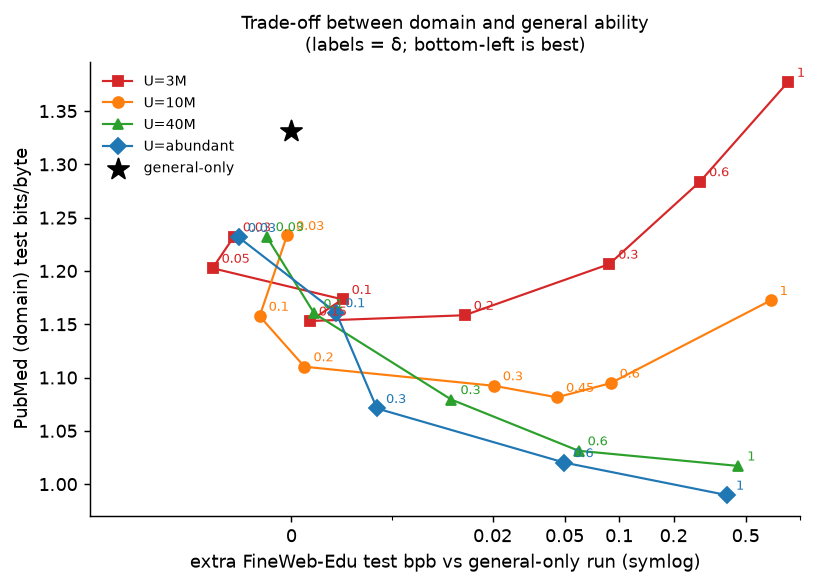
\includegraphics[width=0.85\textwidth]{fig2_tradeoff.png}
\caption{Domain against general test \bpb{} for the mixtures at each $U$; the star is the general-only run.}
\label{fig:trade}
\end{figure}

\paragraph{} For completeness, we also investgiated if there was a tradeoff between domain and general performance. As expected, as $\delta$ increases, the general test \bpb{} increases. However, small $\delta$ helps to increase general domain performance, which could be attributed to the PubMed abstracts adding to the diversity of the training data.  

\section{Discussion}
\subsection{Hypotheses.} 
\begin{table}[h]\centering\small
\renewcommand{\arraystretch}{1.2}
\begin{tabular}{@{}l l p{9.8cm}@{}}\toprule
 & Verdict & Evidence \\\midrule
\textbf{H1} (Adding General Data) & Partially supported & Mixing improves domain \bpb{} only when data is scarce (\(+0.128\) at \(U=3\)M), but hurts when data is abundant (\(-0.031\) at \(U=\text{all}\)). See Table~\ref{tab:gain}. \\
\textbf{H2} (Diminishing returns) & Supported & The gain from mixing drops monotonically as \(U\) increases, eventually crossing zero between \(U=20\)M and \(U=40\)M. \\
\textbf{H3} (Optimal \(\delta^*\)) & Supported & For scarce regimes, an optimum exists (e.g., \(\delta=0.45\) at \(10\)M, \(\delta=0.6\) at \(40\)M). At abundance, \(\delta^*=1.0\) (domain-only is best). However, it is more useful to think in terms of a $E^*$ rather than $\delta^*$ \\
\textbf{H4} (Similarity) & Supported & More PubMed-like general data yields better domain \bpb{}. See Section~\ref{sec:sim}. \\\bottomrule
\end{tabular}
\caption{Summary of findings against the four pre-registered hypotheses.}
\label{tab:hypotheses}
\end{table}

\newpage
\subsection{Relation to prior work.} 
\paragraph{}Our finding that heavy repetition of a small domain set hurts, and that an optimal mixture exists, is consistent with the overfitting scaling laws and U-shaped loss curves reported by \cite{spt2026}. The epoch dynamics we observe, where there is improvement up to a point, then diminishes and eventually results in negative returns, mirror the repetition findings of \cite{muennighoff2023dataconstrained}. \\
However, our investigation differs in these aspects: 
\begin{itemize}
\item The models are trained and tested from scratch rather than using a large pretrained model. There is thus also no finetuning step, which differs from the paper's methodology.
\item The models are a lot smaller (300M tokens with approximately 14M parameters vs. 200B+ tokens and multi-billion parameters)
\end{itemize}



\subsection{Limitations.}
\begin{itemize}
\item Most cells are single-seed, and therefore may not be entirely reliable. The best of many configurations is optimistic by roughly $0.003$-$0.005$~\bpb{} which could affect final conclusions. 
\item The learning rate chosen was tuned on one cell U=40M and $\delta=0.3$. We tested 2e-3, 1e-3 and 6e-4, and 1e-3 and 6e-4 were flat within noise. However, for the sake of brevity, we chose to use only one learning rate.
\item Experiment's were only carried out using one domain, one model size (13.9M parameters), one tokenizer and one general corpus. Results may not be applicable outside of this specific scenario. 
\item Evaluation metrics of \bpb{} means that the models are not evaluated on downstream tasks or prediction accuracy. This means that the models may struggle in actual use. 
\begin{itemize}
\item For example, when prompted with \textit{``Clinical and experimental studies have shown that the coronavirus''}, the model generates plausible-sounding but factually incorrect text (e.g., referring to a vaccine being used in the United States in 2011, before the COVID-19 pandemic). A low \bpb{} score simply indicates the model has learned the statistical distribution of the words, not that it has acquired factual knowledge or reasoning abilities.
\end{itemize}
\item The $E^*$ result that was calculated seems to show a possible non-linear relationship. 
\item Similarity is measured by small models on 256-token prefixes instead of the entire document. Pools also came from one FineWeb-Edu sample, and even the top quartile is far from PubMed.
\item Results come from an AMD nightly PyTorch build; exact numbers will not reproduce bit for bit (see the repository's readme).
\end{itemize}

\section{Conclusion}
\paragraph{}In conclusion, when training a model on a narrow domain, it is recommended to mix in general data to the training process if there is a scarcity of unique domain tokens; where the more similar the general data to the narrow domain the better. For small corpora $U\leq10M$, there is evidence for an optimal number of domain epochs $E^*$ however this rule does not seem to hold at $U=20M$ and thus should be taken as a hypothesis.

\paragraph{Reproducibility.} Code, run summaries, the aggregated results table and the commands that regenerate every figure
are in the repository. \texttt{readme.md} lists three reproduction levels from seconds (figures found in the report generated from \texttt{results/results.csv}) to the full experiment grid.

\newpage
\bibliographystyle{plainnat}
\bibliography{references}

\appendix
\section{Additional figures}



\begin{figure}[h]\centering
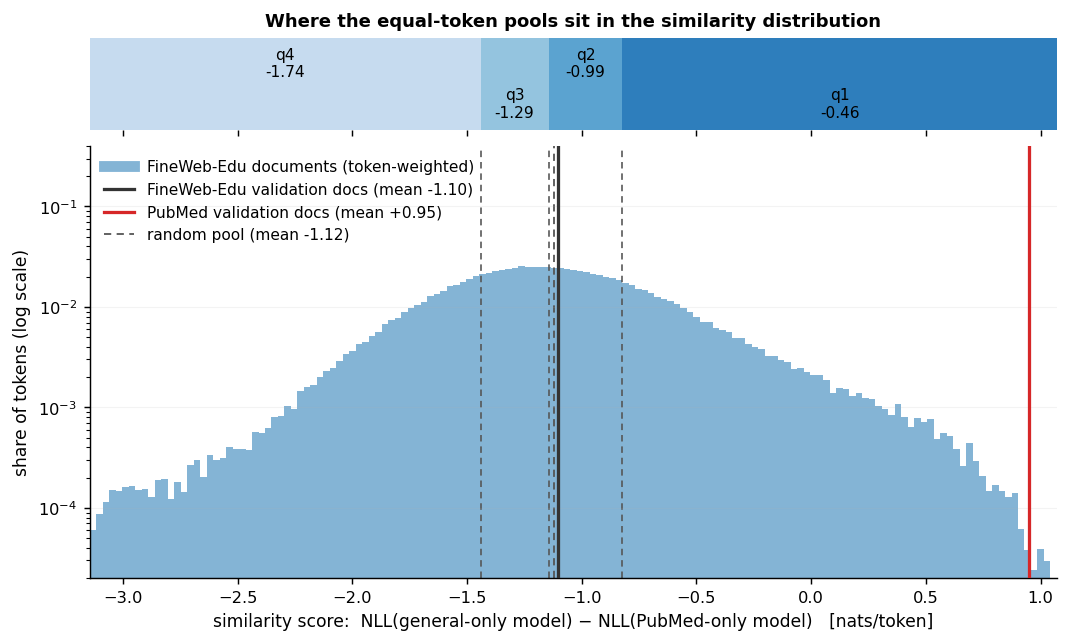
\includegraphics[width=0.85\linewidth]{fig8_sim_distribution.png}
\caption{Distribution of the similarity score over FineWeb-Edu (token-weighted), the equal-token pool boundaries and the validation documents of each corpus.}
\label{fig:dist}
\end{figure}

\end{document}
